
\documentclass[border=10pt,varwidth]{standalone}
\usepackage[left=25mm,right=25mm,top=25mm,bottom=25mm]{geometry}
\usepackage[utf8]{inputenc}
\usepackage[T1]{fontenc}
\usepackage{times}
\usepackage{geometry}
\usepackage{amsmath}
\usepackage{amssymb}
\usepackage{mathrsfs}
\usepackage{amsfonts}
\usepackage{amsthm}
\usepackage{lipsum}
\usepackage{amscd}
\usepackage{graphicx}
\usepackage{fancyhdr}
\usepackage{textcomp}
\usepackage{pgfplots}
\usepackage{txfonts}
\usepackage[all]{xy}
\usepackage{paralist}
\usepackage[colorlinks=true]{hyperref}
\usepackage{array}
\usepackage{tikz}
\usepackage{slashed}
\usepackage{pdfpages}
\usepackage{cite}
\usepackage{url}
\usepackage{amsmath,amsfonts,amssymb}
\usepackage{tikz}
\usepackage{pgfplotstable}
\usetikzlibrary{arrows,matrix,positioning}
\usetikzlibrary{overlay-beamer-styles}
\usetikzlibrary{matrix.skeleton}
\usetikzlibrary{automata,positioning}
\usetikzlibrary{decorations.text}
\usepackage{listings}
\usepackage{multirow}
\usepackage{color}

\begin{document}

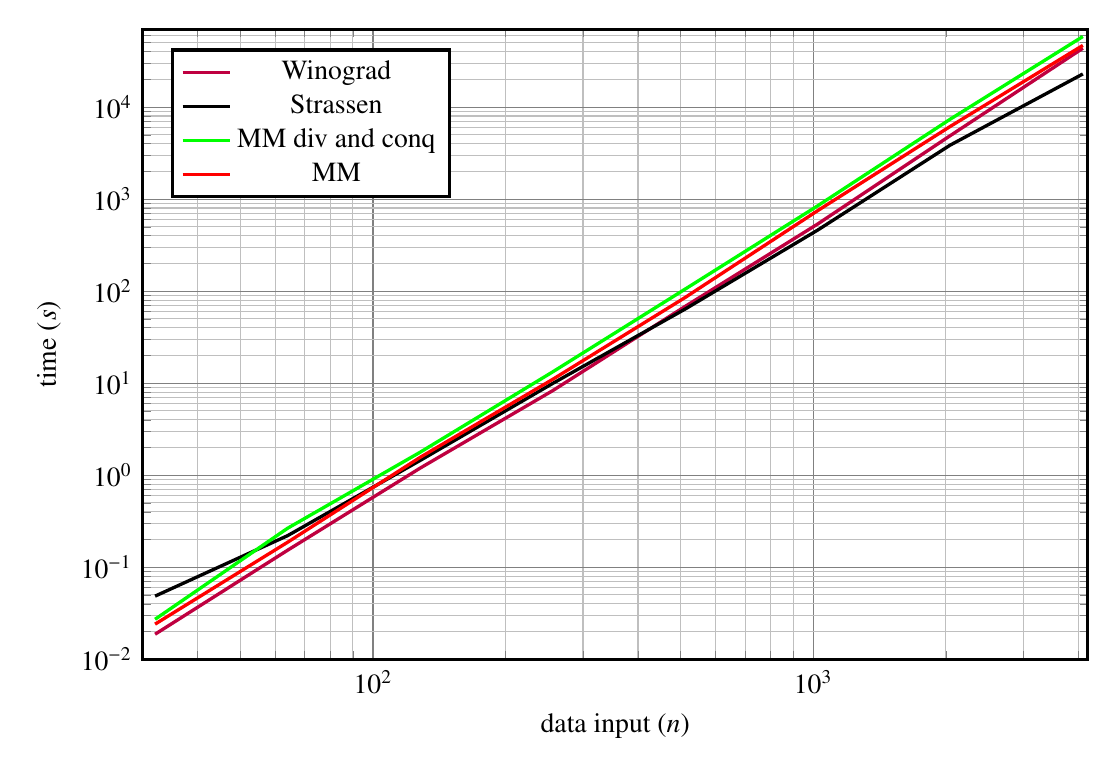
\begin{tikzpicture}
\begin{axis}[
xmode=log, ymode=log,
xmin=30, xmax=4200,
ymin=0.01, ymax=70000,
grid=both,
major grid style={black!50},
xlabel = data input ($n$),
ylabel = {time ($s$)},
legend pos=north west,
very thick,
scale only axis=true,
width=12cm, height=8cm,
       log basis x={10}
]
\addlegendentry{Winograd}
\addplot[    color=purple,
] coordinates {
% (2,   2.7895e-05 )
% (4,   0.000104904)
% (8,   0.000552893)
% (16,  0.0045557  )
(32,  0.0187144  )
(64,  0.153069   )
(128, 1.19476    )
(256, 8.29899    )
(512, 68.3699    )
(1024,537.374    )
(2046,4884.61)
(4096,43597.1)
};
\addlegendentry{Strassen}
\addplot [    color=black,
]coordinates {
  %  (2,2.09808e-05 )
  %  (4,0.000174284 )
  %  (8,0.000943899 )
  % (16,0.00475407  )
  (32,0.0485256   )
  (64,0.220414    )
 (128,1.44718    )
 (256,9.93866    )
 (512,63.961     )
(1024,461.494    )
(2046,3860.57)
(4096,22904.3)
};

\addlegendentry{MM div and conq}
\addplot[    color=green,
] coordinates {
  %  (2,8.10623e-06 )
  %  (4,9.01222e-05 )
  %  (8,0.000729084 )
  % (16,0.00497079  )
  (32,0.02719     )
  (64,0.26528     )
 (128,1.77787      )
 (256,13.27        )
 (512,105.397      )
(1024,847.321      )
(2046,7375.93)
(4096,58466)
};

\addlegendentry{MM}
\addplot [    color=red,
]coordinates {
  %  (2,1.85966e-05)
  %  (4,8.29697e-05 )
  %  (8,0.000547171)
  % (16,0.00305367   )
  (32,  0.0240743 )
  (64,  0.186895 )
 (128,  1.56369 )
 (256,  11.0062 )
 (512,   85.4768)
(1024,750.757 )
(2046,6154.18)
(4096,46813.3)
};
%  \addlegendentry{NumPy}
%  \addplot[    color=blue,
%  ] coordinates {
% %    (2,1.83582e-05 )
% %    (4,7.86781e-06)
% %    (8,1.00136e-05)
% %   (16,5.4121e-05 )
%    (32,4.26769e-05)
%  (64,0.000118494)
%   (128,0.000244141 )
%   (256,0.000695705  )
%   (512,0.00221705   )
%  (1024,0.0188088    )
% (2046,0.215739)
% (4096,1.49159)
%  };

\end{axis}
\end{tikzpicture}

\end{document}
